\section{Developer Incentive Model}
The Developer Incentive Protocol, DIP, including two processes: ranking the DApps and distributing the rewards.

Firstly, constructing a good ranking system can provide third-party developers with a convenient and effective  platform to promote allocations and provide users with a reliable recommendation system. Like the App Store platform for mobile, goods Apps have top positions on the ranking list and thus receive more attention from users. Secondly, users have better experience when their obtain high-quality Apps directly from the ranking lost. Further more, Apps' ranks can be used in keyword search. Just like the search systems in search engines and e-commerce platform,  listing keyword-ralated Apps on the search results according to their ranks is satisfactory to users.

On the other hand, as we shown in Section~\ref{sec:background}, the purpose of DIP is to provide rewards for good DApps' developers, thus further increases developers‘ incentives to design good DApps and promotes the ecosystem development. So the second process of DIP is to design a fair rewarding mechanism, according to DAPPs' ranks,

\subsection{Model Representation}
\label{subsection:parameters}
In this section we introduce necessary notations and symbols in DIP model.

\begin{itemize}
	\item $\mathcal{A}=\{a_1,a_2,\ldots,a_m\}$ represent the set of users that
	  participate the ranking system during a time period. We use voters to
	  denote such users. Note that a user is defined to be a voter only if he
	  invokes some DApp's EOA(External Owned Account) in a time period. Define
	  $$\mathcal{A}^*=\{a_1,a_2,\ldots,a_m,a_{m+1},\ldots,a_{m^*}\}$$
	to be the set of all users in the community during the same time period, i.e., $m*-m$ users do not invoke any DApp.
  \item $\mathcal{D}=\{d_1,\ldots,d_n\}$ represent the set of DApps during a time period.
  \item $e_{ij},i=1,2,\ldots,m, j=1,2,\ldots,n$ represent the times that voter $a_i$ invokes DApp $d_j$. Due to the publicity and decentralization of blockchain, the DIP model is different from the ranking system in traditional centralized application markets. Generally speaking, DIP ranks the DApps according to users' invocation behaviors, in a decentralized environment. The details are shown in the next section.

  \item $\nr_i, i=1,2,\ldots,m$ represent voter $a_i$'s voting capacity during a period of time.
  \cite{Nebulasyellowpaper} proves that user's NR value is an effective measure of his account's value. So in DIP, NR is also used as a significant criterion to decide users' voting capacity.
  \item $\nr_{ij}, i=1,2,\ldots,m,j=1,2,\ldots,n$ represent the contributory value from voter $a_i$ to DApp $d_j$, which can be regarded as the number of votes that $a_i$ willing to vote for $d_j$.

  \item $S_j, j=1,2,\ldots,n$ represent DApp $d_j$'s ranking score, which is determined by its total contributory value from all voters. Intuitively, the ranking scores determine DApps' positions on the ranking list.

  	\item $M$ represents the total amount of the reward pool for developers, granted by the Nabulas group.  The actual reward would be properly reduced according to the participation rate of the whole community during the time period.
   \item $U_j, j=1,2,\ldots,n$ represent the final reward of DApp $d_j$, which is determine by actual total reward and all DApp's ranking scores.
 \end{itemize}
   \begin{figure}
   	\centering
   	%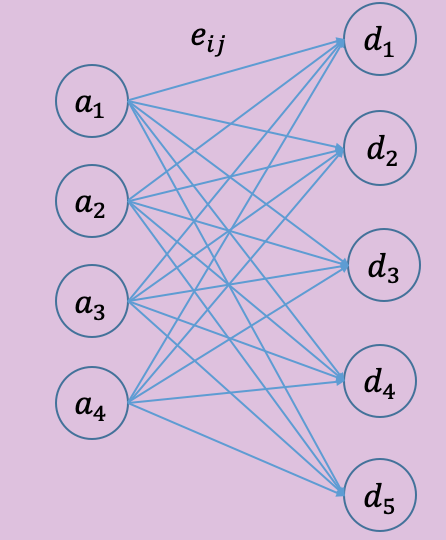
\includegraphics[width = 0.4\textwidth]{../common/m2.png}
   	\begin{tikzpicture}
\pgfmathsetmacro{\XTD}{3.8}
\pgfmathsetmacro{\YTD}{1.2}

\tikzset{
  node/.style={draw, circle, on grid, align=center, minimum height=2ex},
}

\node[node] (d1) at (\XTD, 2*\YTD) {$d_1$};
\node[node] (d2) at (\XTD, \YTD) {$d_2$};
\node[node] (d3) at (\XTD, 0) {$d_3$};
\node[node] (d4) at (\XTD, -1*\YTD) {$d_4$};
\node[node] (d5) at (\XTD, -2*\YTD) {$d_5$};

\node [right=0.05 of d1] {${S}_{1}$};
\node [right=0.05 of d2] {${S}_{2}$};
\node [right=0.05 of d3] {${S}_{3}$};
\node [right=0.05 of d4] {${S}_{4}$};
\node [right=0.05 of d5] {${S}_{5}$};

\node[node] (a1) at (-\XTD, 1.5*\YTD) {$a_1$};
\node[node] (a2) at (-\XTD, 0.5*\YTD) {$a_2$};
\node[node] (a3) at (-\XTD, -0.5*\YTD) {$a_3$};
\node[node] (a4) at (-\XTD, -1.5*\YTD) {$a_4$};

\node [left=0.05 of a1] {${\nr}_{1}$};
\node [left=0.05 of a2] {${\nr}_{2}$};
\node [left=0.05 of a3] {${\nr}_{3}$};
\node [left=0.05 of a4] {${\nr}_{4}$};

\draw[->, >=stealth'] (a1) to (d1);
\draw[->, >=stealth'] (a1) to (d2);
\draw[->, >=stealth'] (a1) to (d3);
\draw[->, >=stealth'] (a1) to (d4);
\draw[->, >=stealth'] (a1) to (d5);

\draw[->, >=stealth'] (a2) to (d1);
\draw[->, >=stealth'] (a2) to (d2);
\draw[->, >=stealth'] (a2) to (d3);
\draw[->, >=stealth'] (a2) to (d4);
\draw[->, >=stealth'] (a2) to (d5);

\draw[->, >=stealth'] (a3) to (d1);
\draw[->, >=stealth'] (a3) to (d2);
\draw[->, >=stealth'] (a3) to (d3);
\draw[->, >=stealth'] (a3) to (d4);
\draw[->, >=stealth'] (a3) to (d5);

\draw[->, >=stealth'] (a4) to (d1);
\draw[->, >=stealth'] (a4) to (d2);
\draw[->, >=stealth'] (a4) to (d3);
\draw[->, >=stealth'] (a4) to (d4);
\draw[->, >=stealth'] (a4) to (d5);

\node at (0, 2*\YTD) {$e_{ij}$};

\end{tikzpicture}

   	\caption{Interactions between voters and DApps \label{fig:interact}}
   \end{figure}
  To sum up, the interactions between voters and DApps can be represented by the bipartite graph in~\ref{fig:interact}.

 \subsection{Voting Action}
 \label{subsection:voting}
  In the centralized App Store\footnote{\url{https://en.wikipedia.org/wiki/App\_store}}, the system can record specific information such as times that a App has been downloaded, which is a key factor for determining its rank. However, in situations of Blockchain, the way that users use DApps is to invoke smart contracts' addresses, e.g., the times that user $a_i$ invokes DApp $d_i$, denoted by  $e_{ij}$. Compared to traditional information about downloads, DIP, that takes information about invocations as the date sources, has the following advantages:

 \begin{itemize}
 	\item The number of invocations are recored on the blockchain, which is hard to be tempered and is more open and transparent, compare to centralized methods such as recording the downloads.
 	\item The number of invocations is more fine-grained compare to the downloads, since downloads only record users' one-shot behavior. But a good DApp should have user stickiness. Therefore the number of invocations are more reasonable to reflect users' real behaviors.

\end{itemize}

 Actually, there are other available informations when users invoke DApps, for example, the amount of gases that has been expended and possible token transfers involved in an invocation. However, DIP takes neither of them into consideration.

 Firstly, the amount of expended gases depend on the executed statements within the smart contracts each time a user invokes a DApp, where the later is not related to the DApp's own quality. Moreover, in the current Nebulas system, the average amount of expended gases during each invocation is at the order of $10^{-8}$ NAS, which is negligible.

 The reason why we do not consider token transfers is the lack of an effective method against manipulation. Intuitively, the wilinesses of users to pay additional tokens when invoking the DApp improve the DApp's {\color{red} identification level}.
  However, in practice, when a user pays tokens to a DApp, the tokens' final destination could belong to the following three cases:

  \begin{enumerate}
  	 \item The tokens finally belongs to the developer of the DApp. In this case, it is believed that the user voluntarily pays to the DApp. Since the DApp's developer has benefited from the user, it is not that meaningful to further increase his rank and reward.
  	\item The DApp itself requires token transfer, such as gambling DApps, which leads  a huge amount of token transfer between the user and the DApp. It's a normal phenomenon. However, the DApp's rank should not be increased accordingly, due to the fact that the user's purpose for paying the token is to gather profits, which does not reflect the DApp's quality.
   \item The DApp's developer commits that all tokens paid to the DApps will be returned to the user. It is actually a kind of manipulation, which would be aggravated if we increases the DApp's rank and reward accordingly.
  \end{enumerate}
  In practice, without analyzing the code of smart contracts, we are not able to determine which case token transfers between users and DApps belongs to and in either case we have explained reasons for not involving DApps' ranks. So the algorithm in DIP will be independent of token transfers.

  In the DIP model, a user $a_i \in \mathcal{A}$ is essentially an account address. As referred in~\cite{Nebulasyellowpaper}, a user can actually control multiple account addresses. Since there is not cost for creating new accounts, the user can forge several addresses which he controls to vote -- the Sybil attack. Similarly, a developer can divide his DApp into several addresses, that is, split his DApp into several low-quality DApps, and obtain all rewards from split DApps. In the meanwhile, a developer can buy over one or more users to vote for his DApp.

  We analyzed all manipulations above when designing DIP and gave corresponding solutions. The details about DIP against manipulation are in Section~\ref{section:properties}.

  \subsection{Sample time interval}
  \label{subsection:interval}
  In Section~\ref{subsection:parameters}, we illustrated that the NR is a significant criterion to determine voters' voting capacities. However, according to th definition in~\cite{Nebulasyellowpaper}, the sampling period of DIP data is much longer than the sampling period of NR data, which means that during the process for recording invocation behaviors, users' NRs may vary, even fluctuate wildly.

  A naive solution is to synchronize the sampling period of NR data and DIP data. However in practice, in a short time period (say, one day), times of invocations are very small for most users. So it is of small significance for ranking the DApps when users behaviors are sparse and the properties discretized  in Section~\ref{section:properties} are not guaranteed to be satisfied.

  So our strategy is to properly extend the sampling period to gather enough invocation behaviors and bound the variation of users' NRs simultaneously. The variation of  an address's NR is shown in Figure~\ref{fig:nr}. Here we divide the whole ranking process of DIP into several time period. According to the data about the variations of NRs, pick integer $t$ such that the variance of NR within $t$ days less than a threshold $\tau$ holds for most users. We take $t$ days as a sampling period, by gather the average NR values of voters and the invocation data in the time period to compute DApp's ranking score and developers' final reward. Then we take the average data over all time periods during a ranking process as the final  results.

  \begin{figure}
  	\label{fig:nr}
  	\centering
  	\pgfplotstableread[col sep=comma]{../common/gateionr.csv}\datatable

\begin{tikzpicture}
  \begin{axis}[
%ticks=none,
ylabel={NR value},
xlabel={date},
%xtick={0,10,20,30,40,50,60},
%xlabel={时间(天)}
legend style={fill=none},
xtick={0, 56},
xticklabels={2018/07/31, 2018/09/25},
extra x ticks={1, 2, ..., 55},
      extra x tick style={
        xticklabels={,,},
      },
%xticklabels from table={\datatable}{record},
width=.75\textwidth,
    ]
\addplot [mark=., color=blue] table [x expr=\coordindex, y=nr, col sep=comma] {../common/gateionr.csv};

\draw[dashed, color=gray] (axis cs:0, 340000000) -- ( axis cs:0,
450000000) ;
\draw[dashed, color=gray] (axis cs:6, 340000000) -- ( axis cs:6,
450000000) ;
\draw[dashed, color=gray] (axis cs:21, 340000000) -- ( axis cs:21,
450000000) ;
\draw[dashed, color=gray] (axis cs:35, 340000000) -- ( axis cs:35,
450000000) ;
\draw[dashed, color=gray] (axis cs:56, 340000000) -- ( axis cs:56,
450000000) ;

\draw[<->, color=gray] (axis cs:0, 445000000) -- node[ color=black, fill=violet!25, anchor=center] {\small $t_1$} (axis cs:6, 445000000);
\draw[<->, color=gray] (axis cs:6, 445000000) -- node[ color=black, fill=violet!25,
anchor=center] {\small $t_2$} (axis cs:21, 445000000);
\draw[<->, color=gray] (axis cs:21, 445000000) -- node[ color=black, fill=violet!25,
anchor=center] {\small $t_3$} (axis cs:35, 445000000);
\draw[<->, color=gray] (axis cs:35, 445000000) -- node[ color=black, fill=violet!25,
anchor=center] {\small $t_4$} (axis cs:56, 445000000);
\end{axis}

\end{tikzpicture}

  	\caption{NR variation graph of an address on Nebulas main net. The main net address is n1Ugq21nif8BQ8uw81SwXHK6DHqeTEmPRhj.}
  \end{figure}



